\documentclass[11pt,a4paper]{article}

\usepackage[utf8]{inputenc}
\usepackage[T1]{fontenc}
\usepackage[margin=1in]{geometry}
\usepackage{booktabs}
\usepackage{amsmath,amssymb}
\usepackage[hidelinks]{hyperref}
\usepackage{caption}
\usepackage{pgfplots}
\pgfplotsset{compat=1.16}

%% Every number, both tables and the figure are generated from the analysis
%% output by sayilar.py. None is typed by hand.
% GENERATED by sayilar.py from sonuc.json and saglamlik.json. Do not edit.
\newcommand{\AllKOne}{12}
\newcommand{\AtSeventeen}{7}
\newcommand{\BetaRatio}{1.6}
\newcommand{\DiscBL}{0.75}
\newcommand{\DiscBestR}{0.56}
\newcommand{\DiscHour}{18:00}
\newcommand{\DiscRefR}{0.18}
\newcommand{\DiscZL}{17.7}
\newcommand{\EarlierHour}{5}
\newcommand{\FxRobustK}{12}
\newcommand{\MaxBestR}{0.69}
\newcommand{\MaxRefR}{0.28}
\newcommand{\MaxZL}{19.1}
\newcommand{\MedBE}{0.82}
\newcommand{\MedBL}{0.86}
\newcommand{\MedBestR}{0.55}
\newcommand{\MedBetaBest}{0.83}
\newcommand{\MedBetaRef}{0.53}
\newcommand{\MedDR}{0.33}
\newcommand{\MedRLate}{0.18}
\newcommand{\MedRefR}{0.22}
\newcommand{\MinBestR}{0.14}
\newcommand{\MinRefR}{0.06}
\newcommand{\MinZL}{5.7}
\newcommand{\NBroad}{9}
\newcommand{\NDaysMax}{597}
\newcommand{\NDaysMin}{596}
\newcommand{\NDropped}{0}
\newcommand{\NFunds}{12}
\newcommand{\NTech}{3}
\newcommand{\PfourK}{12}
\newcommand{\PfourNeed}{10}
\newcommand{\PlaceboMed}{-0.01}
\newcommand{\PlaceboSig}{0}
\newcommand{\PoneK}{7}
\newcommand{\PoneNeed}{7}
\newcommand{\PthreeK}{12}
\newcommand{\PthreeNeed}{7}
\newcommand{\PtwoK}{9}
\newcommand{\PtwoNeed}{7}
\newcommand{\RefKTwo}{12}
\newcommand{\SeasonSame}{8}
\newcommand{\SeasonSameAtSeventeen}{7}
\newcommand{\SignP}{0.0002}
\newcommand{\TechMedBestR}{0.65}
\newcommand{\WindowFirst}{2024-07-08}
\newcommand{\WindowLast}{2026-11-20}
\newcommand{\TabScanRows}{%
AOY & ES & 596 & 2 & 0.075 & 16:00 & 1 & 0.184 & $+0.110$ & 16:00 / 16:00 & -- & \checkmark \\
AFA & ES & 596 & 2 & 0.283 & 17:00 & 1 & 0.691 & $+0.408$ & 17:00 / 17:00 & \checkmark & \checkmark \\
AFV & ES & 596 & 2 & 0.221 & 14:00 & 1 & 0.425 & $+0.204$ & 12:00 / 14:00 & -- & -- \\
AFS & ES & 596 & 2 & 0.121 & 15:00 & 1 & 0.175 & $+0.054$ & 15:00 / 17:00 & -- & -- \\
AFT & NQ & 596 & 2 & 0.229 & 17:00 & 1 & 0.652 & $+0.423$ & 17:00 / 16:00 & \checkmark & \checkmark \\
GBC & ES & 596 & 2 & 0.218 & 17:00 & 1 & 0.571 & $+0.353$ & 17:00 / 16:00 & \checkmark & \checkmark \\
GUH & NQ & 596 & 2 & 0.212 & 17:00 & 1 & 0.632 & $+0.420$ & 17:00 / 16:00 & \checkmark & \checkmark \\
GBG & ES & 596 & 2 & 0.220 & 16:00 & 1 & 0.534 & $+0.314$ & 17:00 / 16:00 & -- & \checkmark \\
YAY & NQ & 596 & 2 & 0.216 & 17:00 & 1 & 0.661 & $+0.445$ & 17:00 / 17:00 & \checkmark & \checkmark \\
ZSF & ES & 596 & 2 & 0.056 & 14:00 & 1 & 0.142 & $+0.086$ & 14:00 / 15:00 & -- & \checkmark \\
ARE & ES & 596 & 2 & 0.168 & 17:00 & 1 & 0.369 & $+0.201$ & 11:00 / 16:00 & \checkmark & -- \\
TMG & ES & 596 & 2 & 0.253 & 17:00 & 1 & 0.603 & $+0.350$ & 17:00 / 16:00 & \checkmark & \checkmark \\
}
\newcommand{\TabLateRows}{%
AOY & 0.64 (0.11) & 0.85 (0.09) & 9.2 & $-0.09$ (0.08) & 0.47 & 0.72 & 16:00 / 18:00 \\
AFA & 0.89 (0.06) & 0.89 (0.05) & 18.4 & $-0.02$ (0.06) & 0.57 & 0.90 & 17:00 / 17:00 \\
AFV & 0.44 (0.07) & 0.67 (0.06) & 11.9 & $+0.05$ (0.05) & 0.44 & 0.62 & 14:00 / 14:00 \\
AFS & 0.22 (0.07) & 0.51 (0.07) & 7.6 & $-0.11$ (0.08) & 0.33 & 0.38 & 15:00 / 13:00 \\
AFT & 0.97 (0.05) & 1.01 (0.06) & 18.4 & $-0.01$ (0.05) & 0.57 & 1.02 & 17:00 / 17:00 \\
GBC & 0.88 (0.06) & 0.84 (0.08) & 10.2 & $+0.07$ (0.04) & 0.53 & 0.87 & 17:00 / 17:00 \\
GUH & 1.04 (0.05) & 1.00 (0.05) & 19.1 & $+0.03$ (0.05) & 0.56 & 1.02 & 17:00 / 17:00 \\
GBG & 0.76 (0.07) & 0.87 (0.07) & 13.1 & $-0.05$ (0.07) & 0.52 & 0.79 & 16:00 / 17:00 \\
YAY & 1.08 (0.06) & 1.05 (0.06) & 17.2 & $+0.05$ (0.06) & 0.60 & 1.12 & 17:00 / 17:00 \\
ZSF & 0.24 (0.05) & 0.23 (0.04) & 5.7 & $+0.04$ (0.04) & 0.16 & 0.25 & 14:00 / 10:00 \\
ARE & 0.46 (0.07) & 0.60 (0.06) & 10.3 & $-0.07$ (0.07) & 0.39 & 0.58 & 17:00 / 17:00 \\
TMG & 0.97 (0.08) & 1.03 (0.06) & 16.2 & $-0.01$ (0.06) & 0.65 & 1.01 & 17:00 / 17:00 \\
}

\captionsetup{font=small}

\title{Which Hour Does a Fund Price?\\
Non-Synchronous Fund Valuation and the Evaluation of Forecasting Systems:\\
Pre-Registered Evidence from T\"urkiye}

\author{Abdullah Faruk Ciftler\\
\small ORCID: \href{https://orcid.org/0009-0001-9310-3812}{0009-0001-9310-3812}}

\date{November 2026}

\begin{document}
\maketitle

\begin{abstract}
A mutual fund's daily price carries a date, not a time. For a fund holding
securities that trade in another time zone, the hour at which they are valued
decides which market session each published return contains, and so how much
of a ``next-day'' price is already fixed when a forecasting system is asked to
predict it. The question arose while auditing a language-model agent whose
one-day fund forecasts missed in a patterned way. We measure the valuation
hour for all \NFunds{} funds on T\"urkiye's fund platform whose names identify
them as foreign-equity funds, under a pre-analysis plan committed before any
of their price series was examined. A fund price dated $t$ is explained best
not by the United States close of day $t-1$ but by futures prices at about
17:00 Istanbul time on that day. The conventional close-to-close alignment
explains a median of \MedRefR{} of the variance of daily fund returns; the
hour-aligned one explains \MedBestR. A test with no hour search confirms it:
the late New York session of day $t-2$ enters the return dated $t$ in all
\NFunds{} funds ($z$ between \MinZL{} and \MaxZL), and the late session of day
$t-1$ in none. An industry directive, located only after the analysis,
prescribes a window of 17:30 to 18:00. Three consequences follow. A system
that predicts such a price after the window is reporting a number already
determined, and a median of \MedRLate{} of its variance is public a full
trading day earlier still, so a no-change baseline is not a fair comparison.
Market betas from daily data are attenuated by a factor of about \BetaRatio.
And under forward pricing the lag is not a trading opportunity. All four
pre-registered criteria are met, one exactly at its threshold.
\end{abstract}

\section{Introduction}

A mutual fund publishes one price per day. When the fund holds securities that
trade while its home market is asleep, that single price has to be struck from
quotes observed at some particular moment, and which moment it is determines
what the fund's daily return means. If the moment is the foreign market's
close, the fund's return lines up with the familiar close-to-close index
return. If it is earlier, part of each foreign session is carried into the
next day's fund return, and anyone comparing the two series date by date is
comparing different things.

The question matters for three groups. Researchers who evaluate fund
performance from daily data estimate betas, tracking errors and alphas whose
values depend on the alignment. Investors read a fund's ``daily return'' on
their platform and compare it with the index move they saw the same day.
Regulators care because a price that is known to lag is, under some dealing
rules, a price that can be traded against.

The literature on this question grew out of the United States, where funds
holding Asian and European shares struck their prices at the New York close
from quotes that were by then many hours old. Those stale prices were
predictable, and because orders could be placed after the information arrived
and still receive the old price, they were also
exploitable~\cite{bhargava1998exploiting,chalmers2001perils,goetzmann2001daytrading,boudoukh2002stale,zitzewitz2003cares}.
The geometry we examine is the reverse: a home market that closes before the
foreign one and values foreign shares while they are still trading.

A fourth group has appeared more recently: people who build and evaluate
forecasting systems. A learned model or a language-model agent asked to
predict ``tomorrow's price'' of such a fund is scored against a number whose
information content was fixed at an hour the benchmark designer may not know.

We study the question for T\"urkiye, whose fund platform lists funds investing
abroad and publishes a dated daily price for each. The hypothesis did not come
from theory. It came from that fourth setting. A language-model agent had been
writing sealed daily forecasts for a handful of assets, scored by a
deterministic engine~\cite{ciftler2026ledger}. An exploratory audit of why its
one-day forecasts for a foreign-equity fund missed in a patterned way found
that the fund's published price tracked United States futures at about 18:00
Istanbul time far better than it tracked the New York close. One fund and an
after-the-fact reading is not evidence. We therefore wrote a pre-analysis plan
fixing the fund universe, the data, the candidate alignments, four hypotheses
and their pass criteria, committed it, and only then downloaded the price
series of \NFunds{} other funds. The originating fund is not in the sample.

\paragraph{Findings.} The pattern replicates across the universe. All four
pre-registered criteria are met. The sharpest of them involves no search over
hours at all and holds in every fund.

\paragraph{Contribution.} We document the valuation hour of foreign-equity
funds in this market, show how large the resulting misalignment is, give a
correction, and set out what the misalignment means for evaluating
forecasting systems on such targets (\S\ref{sec:forecasting}). The hour turns out to be written down, in an industry directive
that neither the regulator's communiqu\'es nor the fund's prospectus text
reproduces. What had not been measured, as far as our search could establish,
is whether published prices follow it and what that does to the return series
(\S\ref{sec:related}).

\section{Institutional background and related work}\label{sec:related}

\paragraph{What the rules say.} We read the rules after the analysis was
finished, and report them in the order in which a data user would meet them.
The securities regulator's communiqu\'e on fund financial reporting requires
exchange-traded assets to be valued at prices formed on the exchange on the
valuation day and foreign-currency assets to be converted at the central
bank's buying rate~\cite{spk2013valuation}. It says nothing about foreign
exchanges and names no hour. The regulator's communiqu\'e on investment funds
and its accompanying guide are equally silent on the
hour~\cite{spk2013funds}. The prospectus of the fund that prompted this study
states only that assets are valued under those rules and under a directive of
the capital markets association.

That directive is where the hour is written~\cite{tspb2026valuation}. Its
article on shares and exchange-traded products listed abroad distinguishes two
cases. If the foreign exchange has finished its trading day by 18:00 Istanbul
time, the closing price is used. If it has not, the price is a weighted
average price obtained from a data vendor at any moment between 17:30 and
18:00 Istanbul time. In both cases the conversion uses the central bank's
indicative buying rate announced at 15:30. The directive was approved by the
regulator, entered into force on 1 March 2024, and has been amended several
times since; we read the text as amended in August 2026 and did not trace
earlier wordings of the article. New York has never finished its day by
18:00 in Istanbul, so United States shares always fall under the second case.

\paragraph{Dealing.} Fund orders in this market are forward priced. The
investment-funds communiqu\'e requires an order to be filled at the unit price
found in the first calculation after the order is given, money-market and
short-term funds excepted~\cite{spk2013funds}. The originating fund's
prospectus sets its daily cut-off at 13:30. We did not read the dealing terms
of each of the \NFunds{} funds in the sample.

\paragraph{Related work.} The early studies established that international
funds priced at the New York close had predictable returns and estimated what
trading on them cost long-term
holders~\cite{bhargava1998exploiting,chalmers2001perils,goetzmann2001daytrading,boudoukh2002stale,zitzewitz2003cares,greene2002dilution}.
A second strand proposed fair-value adjustments that would remove the
predictability~\cite{bhargava2001fairvalue,chua2008fairpricing}. A third is
closest to our purpose: it concerns what stale prices do to performance
evaluation~\cite{qian2011stale}, alongside the related problem of serially
correlated returns in illiquid portfolios~\cite{getmansky2004serial}. More recent work extends the stale-price
question to fixed-income funds~\cite{choi2022sitting}.

We searched for studies of this market specifically: the national citation
index, a general scholarly search engine and a DOI registry, in Turkish and in
English, for stale pricing, valuation time and the timing of fund prices on
the platform. We found none. That is a statement about our search. The
directive itself is public, and those who value these funds apply it; what we
did not find is a measurement of what the window does to the
published return series, or a statement of it in the places where users of
that series would look.

\section{Data and pre-analysis plan}\label{sec:data}

\paragraph{Universe.} The platform's public fund list was read on the day the
plan was written. Every fund whose registered name contains both the words for
``foreign'' and ``equity'' was taken: \NFunds{} funds. The rule was fixed
before any price was downloaded, no fund was added or removed afterwards, and
none fell below the minimum sample. The word ``technology'' appears in the
names of \NTech{} of them.

\paragraph{Fund prices.} Dated daily prices come from the platform's public
price service. The fund return dated $t$ is the ratio of two consecutive
published prices minus one.

\paragraph{Market data.} Hourly bars for E-mini S\&P~500 and E-mini
Nasdaq-100 futures and for the dollar--lira exchange rate, and daily bars for
the corresponding cash indices and the exchange rate, were taken from a public
quote service. A fund with ``technology'' in its name is paired with Nasdaq-100
futures and every other fund with S\&P~500 futures. The pairing was fixed from
the names alone. Because the funds are priced in lira, the exchange-rate
return over the same interval is added to the futures return.

\paragraph{Clock.} All times are Istanbul time, which is three hours ahead of
UTC all year. An hourly bar is labelled by the time it ends. Futures trade
almost around the clock, so the label means the same thing in summer and
winter even though the New York cash session moves by an hour against it.

\paragraph{Window.} The window runs from the first day covered by the hourly
data to a fixed end date written into the plan, \WindowFirst{} to
\WindowLast, giving \NDaysMin{} to \NDaysMax{} fund-price days per fund.

\paragraph{Candidates and reference.} A candidate alignment is a pair $(h,k)$:
the futures-plus-currency return between hour $h$ on trading day $t-k-1$ and
hour $h$ on trading day $t-k$, for every hourly label $h$ and for
$k\in\{0,1,2\}$. The \emph{reference} is the alignment a researcher would
reach for first: the daily close-to-close return of the cash index plus the
daily currency return. We compute it at lags $0$, $1$ and $2$ and keep
whichever lag gives the reference its highest $R^{2}$, so the comparison is
tilted in favour of the conventional approach. Gains in $R^{2}$ are always
computed on identical rows.

\paragraph{Pre-registered hypotheses.}
\begin{description}
  \item[P1, the hour.] The best candidate has $k=1$ and $h$ between 17:00 and
  19:00. Criterion: in at least \PoneNeed{} of \NFunds{} funds.
  \item[P2, size and stability.] The best candidate beats the reference by at
  least $0.05$ in $R^{2}$, and the best hour in each half of the sample lies
  within one hour of the best hour overall. Criterion: both, in at least
  \PtwoNeed{} funds. The hour scan is a multiple comparison, so no $p$-value is
  reported for P1 or P2.
  \item[P3, a test without a search.] Fix the anchor at 18:00, the hour found
  for the originating fund. Let $L_{d}$ be the futures return from 18:00 on day
  $d$ to the New York close of day $d$, the \emph{late session}, and $E_{d}$
  the return from the previous New York close to 18:00 on day $d$. Regress
  \[
    r^{\text{fund}}_{t} = a + b_{E}\,E_{t-1} + b_{L}\,L_{t-2} + \varepsilon_{t}.
  \]
  If the fund is valued near 18:00 on day $t-1$, the late session of day $t-2$
  is still unpriced when the price dated $t-1$ is struck and must appear in the
  return dated $t$: $b_{L}>0$ and close to $b_{E}$. If the fund is valued at
  the New York close, $L_{t-2}$ is already in the previous price and
  $b_{L}=0$. Criterion: $b_{L}>0$ at the one-sided five per cent level with
  heteroskedasticity-robust standard errors, in at least \PthreeNeed{} funds.
  \item[P4, a consequence.] The market beta estimated under the reference
  alignment is smaller than the one estimated at the best candidate.
  Criterion: in at least \PfourNeed{} funds.
\end{description}

The plan also fixed, before the data, that no mechanism would be asserted from
the correlations alone and that no claim about trading would be made without
establishing the dealing rules. Both conditions are taken up in
\S\ref{sec:related} and \S\ref{sec:implications}.

\section{Results}\label{sec:results}

\begin{table}[t]
\centering
\small
\setlength{\tabcolsep}{4.5pt}
\begin{tabular}{llrrrrrrrccc}
\toprule
 & & & \multicolumn{2}{c}{reference} & \multicolumn{4}{c}{best candidate} & & & \\
Fund & Drv. & $n$ & lag & $R^{2}$ & $h$ & $k$ & $R^{2}$ & $\Delta R^{2}$ &
best $h$ by half & P1 & P2 \\
\midrule
\TabScanRows
\bottomrule
\end{tabular}
\caption{Hour scan. ``Drv.'' is the futures contract paired with the fund from
its name (ES: S\&P~500, NQ: Nasdaq-100). The reference is the daily
close-to-close alignment at whichever lag suits it best. $\Delta R^{2}$ is
computed on identical rows. Funds are identified by their public platform
codes.}
\label{tab:scan}
\end{table}

\paragraph{The conventional alignment is two days off.} In all \RefKTwo{}
funds the daily close-to-close return that best explains the fund return dated
$t$ is that of day $t-2$. Even at that lag it explains little: $R^{2}$ between
\MinRefR{} and \MaxRefR, with a median of \MedRefR.

\paragraph{P1 and P2: the hour.} In every fund the best candidate has $k=1$.
In \AtSeventeen{} funds it is 17:00, and in the other \EarlierHour{} it is
earlier in the afternoon (Table~\ref{tab:scan}). P1 required the best hour to
fall between 17:00 and 19:00 in at least \PoneNeed{} funds and is met in
\PoneK: exactly at its threshold, and at the lower edge of the stated range.
We report that plainly. The prediction was written around the 18:00 found for
the originating fund, and the universe turns out to sit an hour earlier. Bar
labels mark the end of an hour, so the two labels that bracket the directive's
window of 17:30 to 18:00 are 17:00 and 18:00. The sample favours the first and
the originating fund the second; in Figure~\ref{fig:curve} the two are the
highest points of most curves. One reading, which hourly bars cannot test, is
that a weighted average price accumulates over the session up to the moment it
is read and therefore reflects a time somewhat before that moment. P2,
which asks for a gain of at least $0.05$ and a stable hour, is met in \PtwoK{}
funds against a criterion of \PtwoNeed. The median gain in $R^{2}$ is \MedDR,
taking the median from \MedRefR{} to \MedBestR. For the \NTech{} technology
funds the median hour-aligned $R^{2}$ is \TechMedBestR.

The \EarlierHour{} funds with earlier best hours are the ones whose names point
away from the United States or toward a single global sector: a European fund,
a fund tracking an index of companies from another group of countries, a
health-care fund, an alternative-energy fund and a multi-country fund. For
these, United States futures are a rough stand-in for the true underlying, and
the plan anticipated that their results would be weaker without removing them
from the denominator.

\begin{figure}[t]
\centering
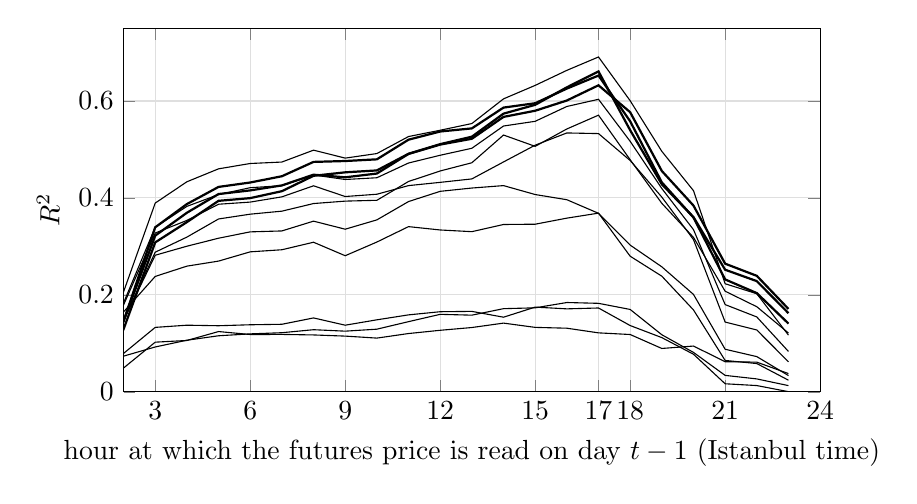
\begin{tikzpicture}
\begin{axis}[width=0.86\textwidth, height=6.2cm,
  xlabel={hour at which the futures price is read on day $t-1$ (Istanbul time)},
  ylabel={$R^{2}$}, xmin=2, xmax=24, ymin=0, ymax=0.75,
  xtick={3,6,9,12,15,17,18,21,24}, grid=major, grid style={gray!25}]
% URETILDI: saglamlik.py - elle duzenleme
\addplot[thin, mark=none] coordinates {(0.0,0.0539) (1.0,0.0005) (2.0,0.0737) (3.0,0.0926) (4.0,0.1065) (5.0,0.1157) (6.0,0.1196) (7.0,0.1220) (8.0,0.1282) (9.0,0.1252) (10.0,0.1293) (11.0,0.1448) (12.0,0.1599) (13.0,0.1582) (14.0,0.1716) (15.0,0.1733) (16.0,0.1843) (17.0,0.1826) (18.0,0.1700) (19.0,0.1178) (20.0,0.0814) (21.0,0.0340) (22.0,0.0267) (23.0,0.0129)}; % AOY
\addplot[thin, mark=none] coordinates {(0.0,0.2655) (1.0,0.0000) (2.0,0.2064) (3.0,0.3894) (4.0,0.4333) (5.0,0.4600) (6.0,0.4710) (7.0,0.4740) (8.0,0.4985) (9.0,0.4821) (10.0,0.4915) (11.0,0.5266) (12.0,0.5396) (13.0,0.5534) (14.0,0.6043) (15.0,0.6321) (16.0,0.6631) (17.0,0.6907) (18.0,0.6005) (19.0,0.4961) (20.0,0.4150) (21.0,0.2230) (22.0,0.2024) (23.0,0.1170)}; % AFA
\addplot[thin, mark=none] coordinates {(0.0,0.1837) (1.0,0.0006) (2.0,0.1471) (3.0,0.2818) (4.0,0.3004) (5.0,0.3169) (6.0,0.3300) (7.0,0.3319) (8.0,0.3521) (9.0,0.3355) (10.0,0.3547) (11.0,0.3925) (12.0,0.4136) (13.0,0.4204) (14.0,0.4254) (15.0,0.4070) (16.0,0.3963) (17.0,0.3683) (18.0,0.3027) (19.0,0.2579) (20.0,0.2010) (21.0,0.0879) (22.0,0.0727) (23.0,0.0336)}; % AFV
\addplot[thin, mark=none] coordinates {(0.0,0.0811) (1.0,0.0031) (2.0,0.0793) (3.0,0.1330) (4.0,0.1375) (5.0,0.1364) (6.0,0.1384) (7.0,0.1394) (8.0,0.1525) (9.0,0.1375) (10.0,0.1486) (11.0,0.1588) (12.0,0.1653) (13.0,0.1660) (14.0,0.1540) (15.0,0.1748) (16.0,0.1712) (17.0,0.1730) (18.0,0.1368) (19.0,0.1119) (20.0,0.0776) (21.0,0.0167) (22.0,0.0130) (23.0,0.0004)}; % AFS
\addplot[thick, mark=none] coordinates {(0.0,0.1933) (1.0,0.0097) (2.0,0.1460) (3.0,0.3394) (4.0,0.3873) (5.0,0.4227) (6.0,0.4318) (7.0,0.4447) (8.0,0.4743) (9.0,0.4761) (10.0,0.4796) (11.0,0.5201) (12.0,0.5370) (13.0,0.5434) (14.0,0.5863) (15.0,0.5953) (16.0,0.6255) (17.0,0.6524) (18.0,0.5581) (19.0,0.4321) (20.0,0.3596) (21.0,0.2319) (22.0,0.2037) (23.0,0.1409)}; % AFT
\addplot[thin, mark=none] coordinates {(0.0,0.2100) (1.0,0.0015) (2.0,0.1471) (3.0,0.2881) (4.0,0.3192) (5.0,0.3566) (6.0,0.3665) (7.0,0.3727) (8.0,0.3884) (9.0,0.3934) (10.0,0.3951) (11.0,0.4339) (12.0,0.4556) (13.0,0.4725) (14.0,0.5297) (15.0,0.5064) (16.0,0.5422) (17.0,0.5707) (18.0,0.4788) (19.0,0.3889) (20.0,0.3186) (21.0,0.2076) (22.0,0.1756) (23.0,0.1213)}; % GBC
\addplot[thick, mark=none] coordinates {(0.0,0.1951) (1.0,0.0074) (2.0,0.1456) (3.0,0.3222) (4.0,0.3694) (5.0,0.4080) (6.0,0.4155) (7.0,0.4258) (8.0,0.4479) (9.0,0.4425) (10.0,0.4503) (11.0,0.4907) (12.0,0.5100) (13.0,0.5220) (14.0,0.5671) (15.0,0.5798) (16.0,0.6009) (17.0,0.6323) (18.0,0.5768) (19.0,0.4556) (20.0,0.3842) (21.0,0.2644) (22.0,0.2393) (23.0,0.1710)}; % GUH
\addplot[thin, mark=none] coordinates {(0.0,0.2038) (1.0,0.0001) (2.0,0.1793) (3.0,0.3276) (4.0,0.3536) (5.0,0.3870) (6.0,0.3914) (7.0,0.4022) (8.0,0.4250) (9.0,0.4029) (10.0,0.4076) (11.0,0.4254) (12.0,0.4321) (13.0,0.4392) (14.0,0.4742) (15.0,0.5088) (16.0,0.5340) (17.0,0.5327) (18.0,0.4772) (19.0,0.4017) (20.0,0.3141) (21.0,0.1440) (22.0,0.1276) (23.0,0.0620)}; % GBG
\addplot[thick, mark=none] coordinates {(0.0,0.1918) (1.0,0.0064) (2.0,0.1292) (3.0,0.3083) (4.0,0.3501) (5.0,0.3940) (6.0,0.3996) (7.0,0.4139) (8.0,0.4456) (9.0,0.4528) (10.0,0.4567) (11.0,0.4911) (12.0,0.5109) (13.0,0.5263) (14.0,0.5738) (15.0,0.5920) (16.0,0.6281) (17.0,0.6609) (18.0,0.5397) (19.0,0.4282) (20.0,0.3604) (21.0,0.2519) (22.0,0.2284) (23.0,0.1623)}; % YAY
\addplot[thin, mark=none] coordinates {(0.0,0.0727) (1.0,0.0001) (2.0,0.0492) (3.0,0.1025) (4.0,0.1060) (5.0,0.1244) (6.0,0.1183) (7.0,0.1185) (8.0,0.1174) (9.0,0.1150) (10.0,0.1109) (11.0,0.1203) (12.0,0.1270) (13.0,0.1327) (14.0,0.1418) (15.0,0.1330) (16.0,0.1313) (17.0,0.1217) (18.0,0.1183) (19.0,0.0895) (20.0,0.0945) (21.0,0.0622) (22.0,0.0613) (23.0,0.0377)}; % ZSF
\addplot[thin, mark=none] coordinates {(0.0,0.1437) (1.0,0.0005) (2.0,0.1649) (3.0,0.2381) (4.0,0.2593) (5.0,0.2697) (6.0,0.2888) (7.0,0.2931) (8.0,0.3086) (9.0,0.2808) (10.0,0.3090) (11.0,0.3408) (12.0,0.3339) (13.0,0.3304) (14.0,0.3452) (15.0,0.3458) (16.0,0.3583) (17.0,0.3686) (18.0,0.2798) (19.0,0.2386) (20.0,0.1690) (21.0,0.0648) (22.0,0.0584) (23.0,0.0241)}; % ARE
\addplot[thin, mark=none] coordinates {(0.0,0.2358) (1.0,0.0001) (2.0,0.1836) (3.0,0.3395) (4.0,0.3826) (5.0,0.4069) (6.0,0.4211) (7.0,0.4252) (8.0,0.4474) (9.0,0.4380) (10.0,0.4416) (11.0,0.4720) (12.0,0.4880) (13.0,0.5024) (14.0,0.5483) (15.0,0.5580) (16.0,0.5886) (17.0,0.6034) (18.0,0.5168) (19.0,0.4194) (20.0,0.3346) (21.0,0.1800) (22.0,0.1545) (23.0,0.0833)}; % TMG

\end{axis}
\end{tikzpicture}
\caption{$R^{2}$ of the fund return dated $t$ on the futures-plus-currency
return between hour $h$ of day $t-2$ and hour $h$ of day $t-1$, one line per
fund; thick lines are the technology funds. Explanatory power rises through
the Istanbul day, peaks near 17:00 and collapses through the New York
afternoon. Hours before 02:00 are omitted: the futures market's daily
maintenance break falls there.}
\label{fig:curve}
\end{figure}

\paragraph{P3: the late session.} Table~\ref{tab:late} gives the test that
involves no search. The coefficient on the late New York session of day $t-2$
is positive and significant in all \PthreeK{} funds, with $z$ between \MinZL{}
and \MaxZL. Its median is \MedBL, against \MedBE{} for the coefficient on the
return from that close to 18:00 on day $t-1$. The two are of the same size, as
valuation near 18:00 implies and valuation at the close forbids. A sign test
across funds gives $p=\SignP$.

\paragraph{P4: betas.} The reference alignment gives a smaller beta than the
best candidate in all \PfourK{} funds. The median beta rises from \MedBetaRef{}
to \MedBetaBest, a factor of about \BetaRatio.

\begin{table}[t]
\centering
\small
\begin{tabular}{lccccccc}
\toprule
 & \multicolumn{3}{c}{P3 (pre-registered)} & placebo & \multicolumn{2}{c}{beta} & best $h$ \\
Fund & $b_{E}$ (s.e.) & $b_{L}$ (s.e.) & $z_{L}$ & $b$ on $L_{t-1}$ (s.e.) &
ref. & best & summer / winter \\
\midrule
\TabLateRows
\bottomrule
\end{tabular}
\caption{Left: the regression of the fund return dated $t$ on the return from
the New York close of day $t-2$ to 18:00 on day $t-1$ ($E$) and on the late
session of day $t-2$ ($L$), with robust standard errors. Right: three checks
that were \emph{not} pre-registered. The placebo adds the late session of day
$t-1$, which occurs after any valuation near 18:00. ``Summer / winter'' is the
best hour at $k=1$ when the United States is on daylight and on standard
time.}
\label{tab:late}
\end{table}

\section{Checks that were not pre-registered}\label{sec:robust}

The following were run after the main results were seen. They are exploratory
and are reported as such.

\paragraph{Placebo.} If valuation happens near 18:00 on day $t-1$, the New
York session that follows it cannot be in the price dated $t$. Adding
$L_{t-1}$ to the P3 regression gives a coefficient indistinguishable from zero
in every fund: \PlaceboSig{} of \NFunds{} exceed two standard errors in either
direction, and the median coefficient is $\PlaceboMed$.

\paragraph{Currency.} Adding the exchange-rate return to the P3 regression
leaves $b_{L}$ positive and significant in \FxRobustK{} funds.

\paragraph{Whose clock.} If funds were valued at a fixed point of the New York
session, the best Istanbul hour would shift by one hour between United States
summer and winter time. Splitting the sample by that calendar, the best hour is
the same in both halves for \SeasonSame{} funds, and for all
\SeasonSameAtSeventeen{} of the funds whose overall best hour is 17:00 it is
17:00 in both. The valuation moment follows the Istanbul clock, not the New
York one. In winter, 17:00 in Istanbul is before the New York cash open.

\paragraph{How much is known in advance.} The late session of day $t-2$ alone,
which is public a full trading day before the price dated $t$ is struck,
explains a median of \MedRLate{} of the variance of the fund return dated $t$.

\paragraph{The originating fund.} The fund that prompted the study is managed
by a different company and was excluded from the sample. Run through the same
code it gives a best hour of \DiscHour, an hour later than the universe, with
an hour-aligned $R^{2}$ of \DiscBestR{} against \DiscRefR{} for its best daily
alignment, and a late-session coefficient of \DiscBL{} ($z=\DiscZL$). Its hour
is the reason P1's range was centred where it was.

\section{Consequences for evaluating forecasting systems}\label{sec:forecasting}

The result began as a problem in evaluating a forecasting agent, and it bears
on any system scored against prices of this kind. We ran no forecasting
experiment for this paper; what follows is implied by the alignment result
and uses only numbers already reported.

\paragraph{A next-day target that is already determined.} The price dated $t$
is struck from quotes read near 17:00 to 18:00 on day $t-1$ and published the
next morning. Between those two moments the target does not yet exist as a
published number, and it can no longer change. A system run in that interval
with access to market data is not forecasting the price dated $t$. It is
reconstructing it. Futures and the exchange rate at the valuation hour alone
account for a median of \MedBestR{} of the variance of the fund return. Part
of the remainder is the gap between a broad futures contract and the fund's
actual holdings, which waiting does not reveal.

\paragraph{Leakage a full day earlier.} Even a system run before the valuation
window holds part of the answer. The late New York session of day $t-2$ is
public by the morning of day $t-1$ and explains a median of \MedRLate{} of the
variance of the return dated $t$. A model given the most recent
close-to-close index return as a feature therefore carries information about
the target that a naive reading of the dates says it should not have. In a
supervised setting this is target leakage through a timestamp convention, and
it will appear as predictive skill.

\paragraph{Baselines must share the information set.} A no-change baseline,
or a drift estimated from past fund returns, sees none of this. A system that
reads the session will beat both without any ability to forecast. The fair
comparator is the mechanical one: the futures-plus-currency return over the
interval the price reflects, up to whatever moment the system was run. Skill
is what remains after that.

\paragraph{Tool-using agents make the information set harder to fix.} For a
model with a fixed training cut-off, the evaluator controls what the model can
know. For an agent that retrieves data when it runs, the information set is
set by the clock at run time and by what the agent chose to look up. Two runs
of the same agent on the same day, one at noon and one in the evening, face
different problems under the same label. A benchmark built on such targets
should record the run time of every prediction and score it against the
baseline available at that time.

\paragraph{Recommendations.} State the valuation hour of every target, or
measure it as we do here. Timestamp each prediction and define its
information set relative to that hour, not to the publication date. Give
baselines the same information. Report instruments with delayed publication
separately from those quoted continuously, since pooling them mixes forecasts
with reconstructions.

\section{What this does and does not imply}\label{sec:implications}

\paragraph{For anyone using daily fund returns.} A foreign-equity fund return
dated $t$ on this platform spans roughly 17:00 on day $t-2$ to 17:00 on day
$t-1$. It contains the whole New York cash session of day $t-2$ and none of
day $t-1$'s. Regressing it on the same-dated index return, or on the
previous day's, measures almost nothing. Using lag two recovers part of the
relationship; aligning by hour recovers most of it. Betas, tracking errors and
any alpha estimated from misaligned daily data are biased, the betas toward
zero. The correction is mechanical: build the benchmark return between the
valuation hours and include the currency leg.

\paragraph{For investors.} The daily return displayed for such a fund is not
the fund's response to that day's market. It is the response to a session that
closed two trading days before the date shown.

\paragraph{For trading: no claim.} A stale price is exploitable only if an
order can be executed at it after the information it omits has become public.
Here it cannot, under the rules we read. Orders are forward priced, and the
one cut-off we verified is 13:30. An investor who orders before the cut-off on
day $d$ receives the price struck that evening, which already contains
everything the previous New York session did. The information the published
price lags is inside the price she deals at. This is the opposite of the
setting in which stale fund prices were first
studied~\cite{chalmers2001perils,zitzewitz2003cares}, where the stale price
was the dealing price. We did not verify the cut-off of each fund in the
sample, and a fund that accepted orders after its valuation window would be a
different case.
We therefore make no claim that the lag can be traded on. What we establish is
when the price is struck, not that anyone can deal against it.

\section{Limitations}\label{sec:limits}

\paragraph{Correlation, not an audit.} We infer the valuation hour from which
futures prices the fund price moves with. That is evidence about what the
price reflects. It is not an audit of any fund's procedure, and we did not
read the valuation documents of the funds in the sample.

\paragraph{The rule was found late.} The pre-analysis plan was written without
knowledge of the directive. Its hour range came from one fund, not from the
rule. Had we read the directive first, the hypothesis would have been a test
of compliance with a stated window, and a sharper one. We have not rewritten
the plan to look as though it was.

\paragraph{One regime.} The whole window lies after the directive entered
into force. We cannot say what the valuation hour was before it.

\paragraph{Hourly resolution.} Bars are one hour wide, so the moment is
located to within about thirty minutes. We cannot distinguish a price read at
17:30 from one read at 17:59, nor say why the sample fits the 17:00 bar better
than the 18:00 one. Finer bars from the same source cover too few days to
meet the plan's minimum sample.

\paragraph{A proxy for the underlying.} Each fund is paired with a broad
futures contract chosen from its name. The funds' actual holdings are not
used. For funds that are not predominantly invested in the United States the
proxy is poor, and their results are weaker for that reason.

\paragraph{One window, one data vendor.} The window is a little over two
years, bounded by the availability of hourly bars from a single public
source, whose historical bars can be revised. The return series computed from
the bars as downloaded are archived with the code.

\paragraph{P1 passed at its threshold.} \PoneNeed{} of \NFunds{} is the
pre-registered criterion and also the count obtained. The hour range was set from one fund;
the universe sits at its lower edge. A plan written without that fund in mind
would have centred the range differently, and we cannot rewrite it now.

\paragraph{The universe is small and name-defined.} The \NFunds{} funds are
every fund the naming rule selects, not a sample from a larger population. Funds that
hold foreign equities under other names, including the originating fund, are
outside it.

\section{Data and code availability}

The pre-analysis plan, the analysis code, the archived fund-price downloads,
the market return series the analysis reads, and the scripts that generate
every number, table and figure in this paper are at
\url{https://github.com/farukciftler/fund-valuation-hour}. All inputs are
public.

Three things about that archive should be stated. First, the plan was committed
to the author's private working repository, which also holds unrelated personal
records and is not public. The commit precedes the download record by less
than two minutes. Both timestamps are the author's own, and a reader cannot
verify their order. Second, the originating fund is one of the assets of the
anonymised dataset cited in the introduction, so its code and price series are
withheld. The five figures reported for it in Section~\ref{sec:robust} are
archived as numbers and cannot be regenerated from the public files. Third,
the quote service's bars are not redistributed. The archive holds the return
series computed from them, unrounded, and the analysis reads those; the bars
can be downloaded again with the same code, but may by then have been revised.

\paragraph{Use of AI in preparing this manuscript.} The analysis code and this
manuscript were drafted with language-model assistance under the author's
direction. Every number in the text and tables is generated from the analysis
output by a script and none is typed by hand. The author is responsible for
the content.

\bibliographystyle{plain}
\bibliography{refs}

\end{document}
